\documentclass[11pt,letterpaper]{article}
\usepackage[T1]{fontenc}
\usepackage{fullpage}
\usepackage[top=2cm, bottom=4.5cm, left=2.5cm, right=2.5cm]{geometry}
\usepackage{amsmath,amsfonts,amssymb}
\usepackage{lastpage}
\usepackage[inline]{enumitem}
\usepackage{fancyhdr}
\usepackage{mathrsfs}
\usepackage{xcolor}
\usepackage{graphicx}
\usepackage{subcaption}
\usepackage{appendix}
\usepackage{hyperref}
\usepackage{titlesec}
\usepackage{fancyvrb}
\hypersetup{colorlinks=true, linkcolor=blue, linkbordercolor={0 0 1}}

%\renewcommand{\arraystretch}{1.5}
\titlespacing*{\section}{0pt}{0.65\baselineskip}{0.5\baselineskip}

\setlength{\parindent}{0.0in}
\setlength{\parskip}{0.05in}

\newcommand{\qrf}{\texttt{QRFactor}}

\pagestyle{fancyplain}
\lhead{}
\chead{GPU Solutions for PSCAD: IT17112}
\rhead{}
\cfoot{\small\thepage}
\headsep 32pt

%%%%%%%%%%%%%%%%%%%%%%%%%%%%%%%%%%%%%%%%%%%%%%%%%%%%%%%%%%%%%%%%%%%%%%%%%%%%%%%
%%%%%%%%%%%%%%%%%%%%%%%%%%%%%%%%%%%%%%%%%%%%%%%%%%%%%%%%%%%%%%%%%%%%%%%%%%%%%%%

\begin{document}
\begin{center}
    {\Large \bf Monthly Summary: December, 2020 \& January, 2021}
\end{center}

During this period, the full functionality -- both device-side and host-side functions -- of \qrf~was incorporated into a DLL (Dynamic Link Library) version and documentation was created to reflect these changes. To produce a DLL that is compiler independent, wrapper functions were created that take and return QRFactor-type pointers. In \S\!\!~\ref{sec: client}, we show how the QRFactor DLL is used by a client program.

The inclusion of GPU functions meant that the DLL template available in Visual Studio was not immediately applicable. Instead, customization of the template was required. See \S\!\!~\ref{sec: gpu dll} for details.

Following a December meeting with the UW and MHI teams, additional changes to QRFactor were discussed that would allow for better integration will future PSCAD EMT updates. These additional changes are outlined in \S\!\!~\ref{sec: additions} and are currently being implemented.

\section{Using QRFactor DLL Within a Client Program}
\label{sec: client}

As mentioned above, the QRFactor DLL was written to be compiler-independent and does this by taking and returning typed pointers, which are then converted into void types upon compilation. With this structure in mind, a client program uses the QRFactor DLL in the following way:
\begin{verbatim}
    #include "qrgpu.h"  // Header file for QRFactor library

    int main()
    {
        double* inPtr;  // Pointer to column-major dense matrix  
        int* rPtr;      // Pointer to number of rows
        int* cPtr;      // Pointer to number of columns
        int* nnz;       // Pointer to total number of non-zero values

        /*
        * Create an instance of QRFactor with the total number of
        * non-zero values as an input
        */
        QRFactor* qr = QR_Create(*nnz);

        /*
        * Build the non-zero entries with the input matrix. Repeat as
        * many times as required until all subsystems have been read in
        */ 
        qr = QR_buildTriplets(qr, inPtr, *rPtr, *cPtr);
        
        /*
        * Assuming all subsystems have been read in, now build the
        * full system sparse matrix and convert to CSR storage
        */
        qr = QR_buildSparseMatrix(qr);

        /*
        * Use GPU-based factoring method on the full system matrix
        */
        qr = QR_factor(qr);
    
        /* 
        * The matrix has been factored and is held on the GPU. Solve 
        * the linear system for each set of input data.
        */
        double* b1;      // Pointer to input vector
        double* x1;      // Pointer to variable vector
        qr = QR_solve(qr, const_cast<double*>(b1), x1);

        double* b2;      // Pointer to input vector
        double* x2;      // Pointer to variable vector
        qr = QR_solve(qr, const_cast<double*>(b2), x2);

        /*
        * Memory cleanup
        */
        QR_delete(qr);

        return 0;
    }
\end{verbatim}


\section{Creating a DLL with Device-side Functions in Microsoft Visual Studio 2019}
\label{sec: gpu dll}
Beginning with a CUDA runtime template project in VS2019, several adjustments are required to create a DLL with CUDA functions. In particular, the project's General Properties page must be changed so that the Configuration Type is Dynamic Library (.dll); see figure~\ref{fig: gen props}.

\begin{figure}[h]
    \centering
    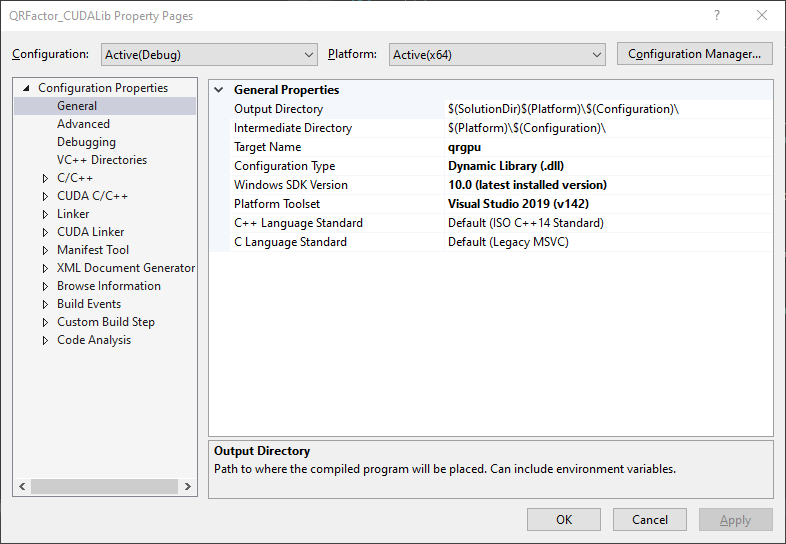
\includegraphics[width=0.75\textwidth]{DLL_GeneralProperties.png}
    \caption{A snapshot of the Configuration Properties $\to$ General tab for a DLL project.}
    \label{fig: gen props}
\end{figure}

--------------------------------------------------------\\

This VS2019 template does not come with the required header files that guide the compilation into the DLL. Those files can be found in the DLL template project

--------------------------------------------------------\\

The user then creates a new header file that contains the library contents. Within the header file, any function declarations that are accessible to the client program must be wrapped with import/export macros and the \verb+EXTERN+ keyword:
\begin{verbatim}
    #ifdef QRGPU_EXPORTS
    #define QRGPU_API __declspec(dllexport)
    #else
    #define QRGPU_API __declspec(dllimport)
    #endif

    #ifdef __cplusplus			
    #define EXTERN
    #else
    #define EXTERN extern "C"
    #endif

    EXTERN QRGPU_API function;      // Example function declaration
\end{verbatim}


\section{Pending Additions}
\label{sec: additions}
The following additions to the QRFactor DLL were discussed and are currently being implemented:
\begin{itemize}
    \item Check whether a GPU is connected and return an error if the library is not able to run on the existing architecture.
    \item Use a map container to trace the positions of the submatrices within the larger full system matrix. This can be used later to quickly identify subsystems with values that change within the EMT system being studied, allowing the system matrix to be rapidly rapidly updated without requiring reassembly.
\end{itemize}


%%%%%%%%%%%%%%%%%%%%%%%%%%%%%%%%%%%%%%%%%%%%%%%%%%%%%%%%%%%%%%%%%%%%%%%%%%%%%%%
%%%%%%%%%%%%%%%%%%%%%%%%%%%%%%%%%%%%%%%%%%%%%%%%%%%%%%%%%%%%%%%%%%%%%%%%%%%%%%%































\end{document}
